\documentclass[aspectratio=169,12pt,t]{beamer}

% --- Theme: Metropolis (modern, clean) ---
\usetheme[progressbar=frametitle,numbering=fraction,block=fill]{metropolis}

% --- Fira Sans font (install texlive-fonts-extra if missing) ---
\IfFileExists{FiraSans.sty}{\usepackage[sfdefault]{FiraSans}}{}

% --- Light background with warm accent ---
\definecolor{mDarkTeal}{RGB}{35,55,59}
\definecolor{mLightBrown}{RGB}{235,228,216}
\definecolor{mAccent}{RGB}{140,70,20}

\setbeamercolor{normal text}{fg=mDarkTeal,bg=white}
\setbeamercolor{alerted text}{fg=mAccent}
\setbeamercolor{frametitle}{bg=mDarkTeal,fg=white}
\setbeamercolor{progress bar}{fg=mAccent,bg=mLightBrown}
\setbeamercolor{title separator}{fg=mAccent}
\setbeamercolor{progress bar in head/foot}{fg=mAccent,bg=mLightBrown}
\setbeamercolor{progress bar in section page}{fg=mAccent,bg=mLightBrown}

% --- Packages ---
\usepackage[utf8]{inputenc}
\usepackage{amsmath,amssymb,amsthm}
\usepackage{mathrsfs}
\usepackage{tikz}
\usetikzlibrary{arrows.meta,positioning,calc,decorations.pathreplacing,shapes,patterns}
\usepackage{pgfplots}
\pgfplotsset{compat=1.18}

% --- Custom colors for content types ---
\definecolor{defcolor}{RGB}{25,85,120}
\definecolor{thmcolor}{RGB}{140,35,35}
\definecolor{proofcolor}{RGB}{35,100,50}
\definecolor{excolor}{RGB}{140,75,10}
\definecolor{remcolor}{RGB}{90,90,90}

% --- Beamer blocks for mathematical content types ---
\newenvironment{defblock}[1]{%
  \setbeamercolor{block title}{bg=defcolor,fg=white}%
  \setbeamercolor{block body}{bg=defcolor!5}%
  \begin{block}{#1}}{\end{block}}

\newenvironment{thmblock}[1]{%
  \setbeamercolor{block title}{bg=thmcolor,fg=white}%
  \setbeamercolor{block body}{bg=thmcolor!5}%
  \begin{block}{#1}}{\end{block}}

\newenvironment{proofblock}[1]{%
  \setbeamercolor{block title}{bg=proofcolor,fg=white}%
  \setbeamercolor{block body}{bg=proofcolor!5}%
  \begin{block}{#1}}{\end{block}}

\newenvironment{exblock}[1]{%
  \setbeamercolor{block title}{bg=excolor,fg=white}%
  \setbeamercolor{block body}{bg=excolor!5}%
  \begin{block}{#1}}{\end{block}}

\newenvironment{remblock}[1]{%
  \setbeamercolor{block title}{bg=remcolor,fg=white}%
  \setbeamercolor{block body}{bg=remcolor!5}%
  \begin{block}{#1}}{\end{block}}

% --- Metadata ---
\title{Chapter 2: Basic Topology}
\subtitle{Section: Connected Sets}
\author{Based on Walter Rudin's \emph{Principles of Mathematical Analysis}}
\date{}

\begin{document}

% =============================================================================
% TITLE AND OUTLINE
% =============================================================================
\begin{frame}
  \titlepage
  \note{
    Welcome back to Chapter 2 of Principles of Mathematical Analysis. This is
    the final section of the topology chapter, and it introduces one last
    structural property that a set in a metric space can have: connectedness.
    Intuitively, a connected set is a set that cannot be broken into two
    pieces that stand apart from each other. We will make this precise using
    the notion of separated sets, and then we will see that the connected
    subsets of the real line have a remarkably simple description: they are
    exactly the intervals, in a broad sense of the word. Let us begin.
  }
\end{frame}

% =============================================================================
\begin{frame}{Outline}
  \tableofcontents
  \note{
    Here is the plan. We first define what it means for two sets to be
    separated, and then what it means for a set to be connected. After a
    short remark that clarifies the difference between disjoint and
    separated, we state the main theorem of the section: a subset of the
    real line is connected if and only if it satisfies a simple order
    condition. We then work through the proof in both directions, and we
    close with a summary of what we have learned.
  }
\end{frame}

% =============================================================================
% MOTIVATION
% =============================================================================

% --- Build 1/3 ---
\begin{frame}{Why This Section Matters}
  \begin{itemize}
    \item So far we have studied \alert{open}, \alert{closed}, \alert{compact}, and \alert{perfect} sets
  \end{itemize}

  \note{
    So far in Chapter 2 we have built up a toolkit of topological properties.
    We studied open sets and closed sets, which capture what it means for a
    set to have no boundary missing or no boundary extra. We studied compact
    sets, which combine closedness with a finiteness-like property. And in
    the previous section we studied perfect sets, which have no isolated
    points.
  }
\end{frame}

% --- Build 2/3 ---
\begin{frame}{Why This Section Matters}
  \begin{itemize}
    \item So far we have studied \alert{open}, \alert{closed}, \alert{compact}, and \alert{perfect} sets
    \item One more key property: whether a set comes in \alert{one piece}
  \end{itemize}

  \note{
    There is one more qualitative property that is fundamental in analysis
    and topology: whether a set comes in one piece or whether it can be split
    into pieces that have nothing to do with each other. A set like the
    interval from 0 to 1 feels like one piece, while a set like the interval
    from 0 to 1 together with the interval from 2 to 3 clearly comes in two
    pieces.
  }
\end{frame}

% --- Build 3/3 ---
\begin{frame}{Why This Section Matters}
  \begin{itemize}
    \item So far we have studied \alert{open}, \alert{closed}, \alert{compact}, and \alert{perfect} sets
    \item One more key property: whether a set comes in \alert{one piece}
    \item Goal: make ``one piece'' precise $\;\Longrightarrow\;$ \alert{connectedness}
  \end{itemize}

  \note{
    Our goal in this section is to turn this intuitive idea of being in one
    piece into a rigorous mathematical definition. The resulting concept is
    called connectedness. It will turn out to be the property that ties
    together many later results, for example the intermediate value theorem
    for continuous functions. Let us see the formal definition.
  }
\end{frame}

% =============================================================================
\section{Separated and Connected Sets}
% =============================================================================

% --- Definition 2.45: Build 1/2 ---
\begin{frame}{Definition 2.45: Separated Sets}
  \begin{defblock}{Definition 2.45 --- Separated Sets}
    Two subsets $A$ and $B$ of a metric space $X$ are \alert{separated} if
    \[
      A \cap \bar{B} = \varnothing \quad \text{and} \quad \bar{A} \cap B = \varnothing.
    \]
    That is, no point of $A$ lies in the closure of $B$, and no point of $B$
    lies in the closure of $A$.
  \end{defblock}

  \note{
    The intuition behind separated sets is this: two sets are separated
    when they sit genuinely apart from each other, with no approach even
    in the limit sense. It is not enough for them to share no elements.
    They must also not be able to reach each other through limit points.
    Formally, as the slide shows, we ask for two conditions: "A" does not
    meet the closure of "B", and "B" does not meet the closure of "A".
    Recall that the closure of a set is the set together with all of its
    limit points. So separation is strictly stronger than disjointness:
    two disjoint sets can still touch through closures, but separated sets
    cannot. A concrete picture is coming up shortly.
  }
\end{frame}

% --- Definition 2.45: Build 2/2 ---
\begin{frame}{Definition 2.45: Connected Sets}
  \begin{defblock}{Definition 2.45 --- Separated Sets}
    Two subsets $A$ and $B$ of a metric space $X$ are \alert{separated} if
    \[
      A \cap \bar{B} = \varnothing \quad \text{and} \quad \bar{A} \cap B = \varnothing.
    \]
  \end{defblock}

  \vspace{0.3em}
  \begin{defblock}{Definition 2.45 --- Connected Set}
    A set $E \subset X$ is \alert{connected} if $E$ is \emph{not} a union of
    two nonempty separated sets.
  \end{defblock}

  \note{
    Now we can define connectedness. Notice that the definition is
    negative: a set "E" is connected precisely when it cannot be split
    into two nonempty separated pieces. This style of definition, where
    the positive property is the absence of a certain decomposition, is
    common and powerful. It tells us exactly how to argue. To show "E" is
    connected, we typically assume for contradiction that such a
    decomposition existed, and derive an impossibility. To show "E" is
    not connected, we exhibit a concrete decomposition into two nonempty
    separated pieces. Both patterns will appear in the proof later in
    this section.
  }
\end{frame}

% --- Diagram: Separated vs. Non-Separated ---
\begin{frame}{Picture: Separated Sets}
  \begin{center}
  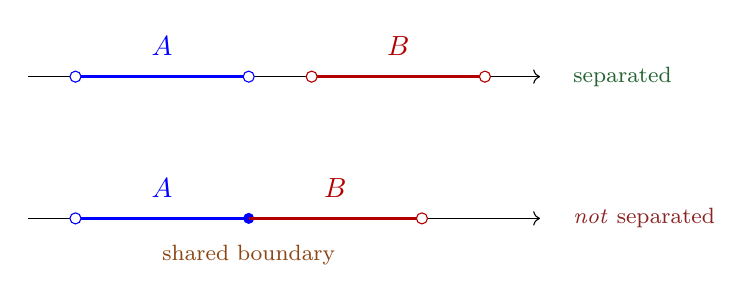
\begin{tikzpicture}[scale=1.0]
    % Top: separated
    \draw[->] (-0.3,1.8) -- (6.2,1.8);
    \draw[very thick, blue] (0.3,1.8) -- (2.5,1.8);
    \draw[blue, fill=white] (0.3,1.8) circle (2pt);
    \draw[blue, fill=white] (2.5,1.8) circle (2pt);
    \node[blue, above=4pt] at (1.4,1.8) {$A$};
    \draw[very thick, red!70!black] (3.3,1.8) -- (5.5,1.8);
    \draw[red!70!black, fill=white] (3.3,1.8) circle (2pt);
    \draw[red!70!black, fill=white] (5.5,1.8) circle (2pt);
    \node[red!70!black, above=4pt] at (4.4,1.8) {$B$};
    \node[right, proofcolor] at (6.5,1.8) {\footnotesize separated};
    % Bottom: not separated
    \draw[->] (-0.3,0) -- (6.2,0);
    \draw[very thick, blue] (0.3,0) -- (2.5,0);
    \fill[blue] (2.5,0) circle (2pt);
    \draw[blue, fill=white] (0.3,0) circle (2pt);
    \node[blue, above=4pt] at (1.4,0) {$A$};
    \draw[very thick, red!70!black] (2.5,0) -- (4.7,0);
    \draw[red!70!black, fill=white] (4.7,0) circle (2pt);
    \node[red!70!black, above=4pt] at (3.6,0) {$B$};
    \node[mAccent, below=6pt] at (2.5,0) {\footnotesize shared boundary};
    \node[right, thmcolor] at (6.5,0) {\footnotesize \emph{not} separated};
  \end{tikzpicture}
  \end{center}

  \vspace{0.5em}
  \alert{Separation} = gap in both directions: neither set touches the other's closure.

  \note{
    This picture shows two scenarios on the real line. In the top row we
    see two blue and red intervals separated by a visible gap. Neither set
    contains a limit point of the other, so they are separated in the sense
    of the definition. In the bottom row, the right endpoint of the blue
    interval and the left endpoint of the red interval coincide at a single
    shared boundary point. The blue set contains this boundary point, and it
    is also a limit point of the red set, so the closure of the red set meets
    the blue set. These two sets are disjoint but not separated. Separation
    requires not just disjointness, but also that no limit-point contact
    exists between the two sets.
  }
\end{frame}

% --- Remark 2.46: Build 1/3 ---
\begin{frame}{Remark 2.46: Disjoint Does Not Mean Separated}
  \begin{remblock}{Remark 2.46 --- Key Fact}
    \begin{itemize}
      \item Separated sets are \alert{always disjoint}.
      \item Disjoint sets \alert{need not be} separated.
    \end{itemize}
  \end{remblock}

  \note{
    The remark clarifies the relationship between the two notions of
    disjointness and separation. If two sets are separated, then the
    closure of each one is disjoint from the other, so in particular the
    sets themselves are disjoint. That direction is easy. The converse,
    however, fails. Two sets can be disjoint without being separated, and
    the next two slides give concrete examples of this distinction on the
    real line.
  }
\end{frame}

% --- Remark 2.46: Build 2/3 ---
\begin{frame}{Remark 2.46: Disjoint but \emph{Not} Separated}
  \begin{remblock}{Example --- $[0,1]$ and $(1,2)$}
    Disjoint, but $1 \in [0,1]$ and $1$ is a limit point of $(1,2)$, so
    \[
      [0,1] \cap \overline{(1,2)} = \{1\} \neq \varnothing.
    \]
  \end{remblock}

  \begin{center}
  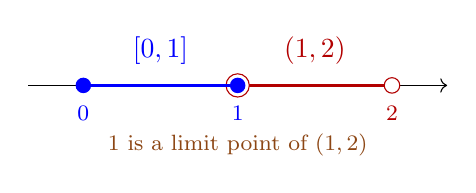
\begin{tikzpicture}[scale=1.4]
    \draw[->] (-0.3,0) -- (3.5,0);
    % (1,2) -- drawn first so the open circle at 1.6 sits under the blue filled dot
    \draw[very thick, red!70!black] (1.6,0) -- (3.0,0);
    \draw[red!70!black, fill=white] (1.6,0) circle (3pt);
    \draw[red!70!black, fill=white] (3.0,0) circle (2pt) node[below=4pt]{\footnotesize $2$};
    \node[red!70!black, above=4pt] at (2.3,0) {$(1,2)$};
    % [0,1] -- drawn last so the filled dot at 1.6 sits on top, showing 1 is in [0,1]
    \draw[very thick, blue] (0.2,0) -- (1.6,0);
    \fill[blue] (0.2,0) circle (2pt) node[below=4pt]{\footnotesize $0$};
    \fill[blue] (1.6,0) circle (2pt) node[below=4pt]{\footnotesize $1$};
    \node[blue, above=4pt] at (0.9,0) {$[0,1]$};
    \node[mAccent, below=14pt] at (1.6,0) {\footnotesize $1$ is a limit point of $(1,2)$};
  \end{tikzpicture}
  \end{center}

  \note{
    Consider the closed interval from 0 to 1 and the open segment from 1 to
    2. These two sets are disjoint: they share no element, because the
    segment from 1 to 2 does not contain the endpoint 1. But the number 1
    belongs to the first set, and 1 is a limit point of the segment from 1
    to 2, since every neighborhood of 1 meets the segment. So 1 lies in the
    closure of the segment, which means the first set meets the closure of
    the second. These sets are therefore disjoint but not separated.
  }
\end{frame}

% --- Remark 2.46: Build 3/3 ---
\begin{frame}{Remark 2.46: \emph{Truly} Separated}
  \begin{remblock}{Example --- $(0,1)$ and $(1,2)$}
    \[
      \overline{(0,1)} = [0,1], \quad \overline{(1,2)} = [1,2].
    \]
    \[
      (0,1) \cap [1,2] = \varnothing, \qquad [0,1] \cap (1,2) = \varnothing.
    \]
    Hence $(0,1)$ and $(1,2)$ \alert{are separated}.
  \end{remblock}

  \begin{center}
  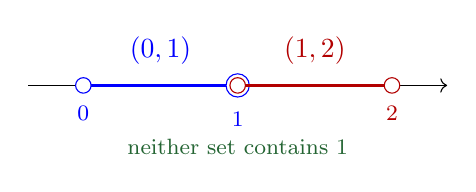
\begin{tikzpicture}[scale=1.4]
    \draw[->] (-0.3,0) -- (3.5,0);
    % (0,1)
    \draw[very thick, blue] (0.2,0) -- (1.6,0);
    \draw[blue, fill=white] (0.2,0) circle (2pt) node[below=4pt]{\footnotesize $0$};
    % Blue open endpoint at 1.6: outer ring (3pt), drawn first
    \draw[blue, fill=white] (1.6,0) circle (3pt) node[below=6pt]{\footnotesize $1$};
    \node[blue, above=4pt] at (0.9,0) {$(0,1)$};
    % (1,2)
    \draw[very thick, red!70!black] (1.6,0) -- (3.0,0);
    % Red open endpoint at 1.6: inner ring (2pt), drawn on top so both circles are visible
    \draw[red!70!black, fill=white] (1.6,0) circle (2pt);
    \draw[red!70!black, fill=white] (3.0,0) circle (2pt) node[below=4pt]{\footnotesize $2$};
    \node[red!70!black, above=4pt] at (2.3,0) {$(1,2)$};
    \node[proofcolor, below=16pt] at (1.6,0) {\footnotesize neither set contains $1$};
  \end{tikzpicture}
  \end{center}

  \note{
    Now replace the closed left interval with the open segment from 0 to 1.
    The two open segments from 0 to 1 and from 1 to 2 are still disjoint,
    but now neither one contains the point 1. The closure of the first
    segment is the closed interval from 0 to 1, and the closure of the
    second segment is the closed interval from 1 to 2. When we check the
    two required intersections, both turn out to be empty. So these two
    segments really are separated. The pivotal difference is whether the
    common boundary point 1 belongs to one of the sets.
  }
\end{frame}

% =============================================================================
\section{Connected Subsets of the Real Line}
% =============================================================================

% --- Theorem 2.47 Statement ---
\begin{frame}{Theorem 2.47: Connected Subsets of $\mathbb{R}^1$}
  \begin{thmblock}{Theorem 2.47}
    A subset $E$ of the real line $\mathbb{R}^1$ is \alert{connected} if and only if it
    has the following property:
    \[
      \boxed{\text{If } x, y \in E \text{ and } x < z < y, \text{ then } z \in E.}
    \]
  \end{thmblock}

  \vspace{0.4em}
  In plain words: $E$ contains every number sitting between two of its own points.

  \note{
    This is the main theorem of the section. It completely characterizes
    connectedness for subsets of the real line. The statement is a
    biconditional: "E" is connected if and only if "E" has the property that,
    whenever it contains two points "x" and "y", it also contains every real
    number sitting strictly between them. Geometrically, this says that "E"
    has no holes: it cannot skip over any point that lies between two of its
    existing points. Sets with this property are exactly the intervals in a
    very broad sense, including open, closed, half-open, and unbounded
    intervals.
  }
\end{frame}

% --- Geometric Intuition ---
\begin{frame}{Picture: The ``No Holes'' Property}
  \begin{center}
  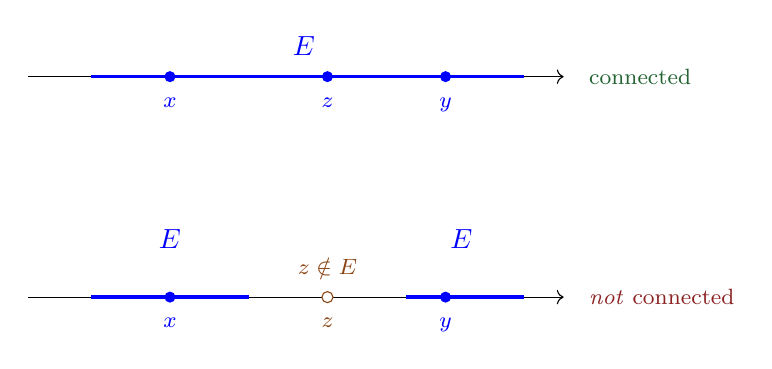
\begin{tikzpicture}[scale=1.0]
    % Connected: one interval
    \draw[->] (-0.3,2.8) -- (6.5,2.8);
    \draw[very thick, blue] (0.5,2.8) -- (6.0,2.8);
    \fill[blue] (1.5,2.8) circle (2pt) node[below=4pt]{\footnotesize $x$};
    \fill[blue] (3.5,2.8) circle (2pt) node[below=4pt]{\footnotesize $z$};
    \fill[blue] (5.0,2.8) circle (2pt) node[below=4pt]{\footnotesize $y$};
    \node[blue, above=4pt] at (3.2,2.8) {$E$};
    \node[right, proofcolor] at (6.7,2.8) {\footnotesize connected};
    % Disconnected: gap
    \draw[->] (-0.3,0) -- (6.5,0);
    \draw[very thick, blue] (0.5,0) -- (2.5,0);
    \draw[very thick, blue] (4.5,0) -- (6.0,0);
    \fill[blue] (1.5,0) circle (2pt) node[below=4pt]{\footnotesize $x$};
    \fill[blue] (5.0,0) circle (2pt) node[below=4pt]{\footnotesize $y$};
    % Gap marker: hollow circle with white fill, indicating z is not in E
    \draw[mAccent, fill=white] (3.5,0) circle (2pt) node[below=4pt]{\footnotesize $z$};
    \node[mAccent, above=4pt] at (3.5,0) {\footnotesize $z \notin E$};
    \node[blue, above=14pt] at (1.5,0) {$E$};
    \node[blue, above=14pt] at (5.2,0) {$E$};
    \node[right, thmcolor] at (6.7,0) {\footnotesize \emph{not} connected};
  \end{tikzpicture}
  \end{center}

  \vspace{0.3em}
  A gap between two points of $E$ immediately breaks connectedness.

  \note{
    This picture shows both scenarios. On the top, the blue set "E" is one
    solid interval, and any three points "x", "z", "y" with "z" between "x"
    and "y" all lie in "E". On the bottom, the blue set "E" consists of two
    disjoint pieces with a gap in the middle. The points "x" and "y" belong
    to "E", but the point "z", marked in orange, sits in the gap and is not
    in "E". Any such missed point between two points of "E" is enough to
    break connectedness, and the theorem says this is the only way
    connectedness can fail on the real line.
  }
\end{frame}

% =============================================================================
\section{Proof of Theorem 2.47}
% =============================================================================

% --- Proof Strategy ---
\begin{frame}{Proof Strategy: Theorem 2.47}
  \textbf{Goal:} Prove the biconditional $E$ connected $\;\Longleftrightarrow\;$ $E$ has the
  in-between property.

  \vspace{0.8em}
  We prove \alert{both directions by contrapositive}:
  \begin{enumerate}
    \item[(A)] If the property \emph{fails}, then $E$ is \emph{not} connected.

          \quad$\leadsto$\; construct an explicit separation of $E$.

    \item[(B)] If $E$ is \emph{not} connected, then the property \emph{fails}.

          \quad$\leadsto$\; use a separation $E = A \cup B$ and take $z = \sup(A \cap [x,y])$.
  \end{enumerate}

  \note{
    Before we dive into the details, here is the high-level plan. We want
    to prove a biconditional, so there are two directions. We prove each by
    contrapositive, which will feel more natural than trying to argue
    directly. In part "A", we assume the in-between property fails, meaning
    we can find two points of "E" and a missing point between them, and we
    use that missing point to explicitly split "E" into two separated pieces.
    In part "B", we assume "E" is not connected, so there is already a
    separation, and we use the supremum trick along with Theorem 2.28 to
    locate a missing point between two points of "E".
  }
\end{frame}

% --- Direction A: Build 1/3 ---
\begin{frame}{Part (A): Property Fails $\;\Longrightarrow\;$ Not Connected}
  \begin{proofblock}{Setup}
    Suppose $\exists\, x, y \in E$ and $z \in (x, y)$ with $z \notin E$.
  \end{proofblock}

  \begin{center}
  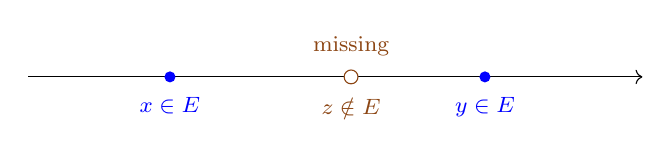
\begin{tikzpicture}[scale=1.0]
    \draw[->] (-0.3,0) -- (7.5,0);
    \fill[blue] (1.5,0) circle (2pt) node[below=4pt]{\footnotesize $x \in E$};
    \draw[mAccent, fill=white] (3.8,0) circle (2.5pt);
    \node[mAccent, below=4pt] at (3.8,0) {\footnotesize $z \notin E$};
    \fill[blue] (5.5,0) circle (2pt) node[below=4pt]{\footnotesize $y \in E$};
    \node[mAccent, above=4pt] at (3.8,0) {\footnotesize missing};
  \end{tikzpicture}
  \end{center}

  \vspace{0.3em}
  Goal: exhibit $E = A_z \cup B_z$ with $A_z, B_z$ \alert{nonempty and separated}.

  \note{
    We start part "A" by assuming the in-between property fails. That means we
    can pick two points "x" and "y" in "E", with "x" less than "y", and a
    point "z" strictly between them that does not belong to "E". The picture
    shows "x" and "y" as solid blue dots in "E", while "z" in the middle is
    shown as an empty orange circle to mark that it is missing. Our goal is
    to use this single missing point to split "E" into two nonempty pieces
    that are separated, thereby showing that "E" is not connected.
  }
\end{frame}

% --- Direction A: Build 2/3 ---
\begin{frame}{Part (A): Constructing the Split}
  \begin{proofblock}{Setup}
    Suppose $\exists\, x, y \in E$ and $z \in (x, y)$ with $z \notin E$.
  \end{proofblock}

  \begin{proofblock}{Step 1 --- Define $A_z$ and $B_z$}
    \[
      A_z = E \cap (-\infty, z), \qquad B_z = E \cap (z, \infty).
    \]
    Since $z \notin E$: \quad $E = A_z \cup B_z$.

    \vspace{0.2em}
    Nonemptiness: \quad $x \in A_z$ (since $x < z$), \quad $y \in B_z$ (since $z < y$).
  \end{proofblock}

  \note{
    We split "E" by cutting at the missing point "z". Define "A" sub "z" to
    be the part of "E" lying strictly to the left of "z", and "B" sub "z" to
    be the part lying strictly to the right of "z". Because "z" itself is
    not in "E", every element of "E" is either strictly less than "z" or
    strictly greater than "z", so the union of "A" sub "z" and "B" sub "z"
    is all of "E". Both pieces are nonempty: "x" lies in "A" sub "z" because
    "x" is less than "z", and "y" lies in "B" sub "z" because "z" is less
    than "y". Next we check separation.
  }
\end{frame}

% --- Direction A: Build 3/3 ---
\begin{frame}{Part (A): Separation and Conclusion}
  \begin{proofblock}{Step 2 --- $A_z$ and $B_z$ are separated}
    \[
      A_z \subset (-\infty, z) \;\Longrightarrow\; \overline{A_z} \subset (-\infty, z],
    \]
    \[
      B_z \subset (z, \infty) \;\Longrightarrow\; \overline{B_z} \subset [z, \infty).
    \]
    Only possible overlap: $\{z\}$. But $z \notin A_z$ and $z \notin B_z$, so
    \[
      A_z \cap \overline{B_z} = \varnothing, \qquad \overline{A_z} \cap B_z = \varnothing.
    \]
  \end{proofblock}

  \begin{proofblock}{Conclusion}
    $E = A_z \cup B_z$ with $A_z, B_z$ nonempty and separated $\;\Longrightarrow\;$ \alert{$E$ is not connected.}
  \end{proofblock}

  \note{
    Now for the separation check. The set "A" sub "z" lives inside the
    half-line to the left of "z", so its closure stays inside the half-line
    to the left of "z" together with "z" itself. Similarly the closure of
    "B" sub "z" lives in the half-line from "z" to the right. The only
    possible overlap between these two closed half-lines is at "z". But "z"
    is not in "A" sub "z" and not in "B" sub "z", so both intersections in
    the definition of separation are empty. We have split "E" into two
    nonempty separated sets, so "E" is not connected. Part "A" is done.
  }
\end{frame}

% --- Direction B: Build 1/4 ---
\begin{frame}{Part (B): Not Connected $\;\Longrightarrow\;$ Property Fails}
  \begin{proofblock}{Setup}
    Suppose $E$ is \emph{not} connected. Then
    \[
      E = A \cup B, \quad A, B \neq \varnothing, \quad A, B \text{ separated}.
    \]
    Pick $x \in A$, $y \in B$. Assume \alert{WLOG $x < y$}.
  \end{proofblock}

  \vspace{0.3em}
  Plan: find $z^\ast$ with $x < z^\ast < y$ and $z^\ast \notin E$.

  \note{
    Now we turn to part "B". Assume "E" is not connected. By definition, we
    can write "E" as the union of two nonempty separated sets, call them
    "A" and "B". Pick any element "x" of "A" and any element "y" of "B".
    Since they come from disjoint sets we have "x" not equal to "y", so
    without loss of generality we can assume "x" is less than "y". If
    instead "y" were less than "x", we could simply swap the names "A" and
    "B" and repeat. Our goal is to find some point strictly between "x" and
    "y" that does not belong to "E".
  }
\end{frame}

% --- Direction B: Build 2/5 ---
\begin{frame}{Part (B): The Key Construction --- $z = \sup(A \cap [x,y])$}
  \begin{proofblock}{Step 1 --- Define $z$}
    \[
      z = \sup\,(A \cap [x, y]).
    \]
    Note: $A \cap [x,y]$ is nonempty ($x$ is in it) and bounded above by $y$.
  \end{proofblock}

  \begin{alertblock}{Recall: Theorem 2.28}
    If $E \subset \mathbb{R}$ is nonempty and bounded above, then $\sup E \in \bar E$.
  \end{alertblock}

  \note{
    Here is the key construction of part "B". The motivating idea: we
    want to find a point sitting right at the boundary between "A" and
    "B". A natural candidate is the rightmost point of "A" that still
    lies inside the interval from "x" to "y". Formally, we take "z" to
    be the supremum of "A" intersected with the closed interval from
    "x" to "y". This supremum is well-defined because the intersection
    is nonempty, since it contains "x", and it is bounded above by "y".
    To analyze where this supremum sits, we invoke Theorem 2.28, shown
    on the slide: for any nonempty bounded-above subset of the reals,
    the supremum always lies in the closure of the set. This gives us
    the leverage we need to trap "z" in a very specific spot. On the
    next slide we pin down exactly where "z" is.
  }
\end{frame}

% --- Direction B: Build 3/5 ---
\begin{frame}{Part (B): Locating $z$}
  \begin{proofblock}{Step 2 --- Locate $z$}
    By Theorem 2.28, $z \in \bar A$. Since $\bar A \cap B = \varnothing$: \; $z \notin B$.

    \vspace{0.3em}
    Three bounds:
    \begin{itemize}
      \item $x \leq z$ \; (since $x \in A \cap [x,y]$),
      \item $z \leq y$ \; (since $y$ is an upper bound),
      \item $z \neq y$ \; (since $y \in B$, $z \notin B$).
    \end{itemize}

    \vspace{0.2em}
    Hence $\;\boxed{x \leq z < y.}$
  \end{proofblock}

  \note{
    Now we apply Theorem 2.28. Since "z" is the supremum of a nonempty set
    that is bounded above, "z" lies in the closure of "A". Because "A" and
    "B" are separated, the closure of "A" is disjoint from "B", so "z" is
    not in "B". That already rules out one location for "z". To pin it
    down further, we collect three bounds shown on the slide. First, "x"
    is less than or equal to "z", because "x" itself belongs to the set
    whose supremum we took. Second, "z" is less than or equal to "y",
    because "y" is an upper bound of that set, and the supremum is the
    least upper bound. Third, "z" is not equal to "y", because "y" lies
    in "B" while "z" does not. Combining these, "z" sits in the half-open
    interval from "x" up to, but not including, "y". Next we split into
    two cases depending on whether "z" belongs to "A".
  }
\end{frame}

% --- Direction B: Build 4/5 ---
\begin{frame}{Part (B): Case 1 --- $z \notin A$}
  \begin{proofblock}{Case 1: $z \notin A$}
    Already know: $z \notin B$. So $z \notin A \cup B = E$.

    \vspace{0.3em}
    And $x \leq z < y$; in fact $x < z$ because $x \in A$ while $z \notin A$.

    \vspace{0.3em}
    $\Longrightarrow\;\;\boxed{x < z < y \text{ and } z \notin E.}$
  \end{proofblock}

  \vspace{0.5em}
  The property $x, y \in E, \; x < z < y \Rightarrow z \in E$ \alert{fails at this $z$}.

  \note{
    Case 1 is the easy case: suppose "z" is not in "A". We already showed
    "z" is not in "B". So "z" is not in the
    union of "A" and "B", which is all of "E". Also, "x" is in "A" but "z"
    is not in "A", so "x" and "z" are different, which together with the
    earlier bound "x" less than or equal to "z" forces "x" strictly less
    than "z". Combining with "z" less than "y", we have found a point
    strictly between "x" and "y" that is not in "E". The in-between
    property fails at this "z". Case 1 is done.
  }
\end{frame}

% --- Direction B: Build 5/5 ---
\begin{frame}{Part (B): Case 2 --- $z \in A$}
  \begin{proofblock}{Case 2: $z \in A$}
    Separation: $A \cap \bar B = \varnothing$, so $z \notin \bar B$.

    \vspace{0.2em}
    Hence some open neighborhood of $z$ misses $B$ entirely: $\exists\, z_1$ with
    \[
      z < z_1 < y \quad \text{and} \quad z_1 \notin B.
    \]
    But $z_1 > z = \sup(A \cap [x,y])$ and $z_1 < y$, so $z_1 \notin A$ either.

    \vspace{0.2em}
    $\Longrightarrow\;\;\boxed{x < z_1 < y \text{ and } z_1 \notin E.}$
  \end{proofblock}

  \vspace{0.3em}
  In both cases the in-between property fails \quad $\blacksquare$

  \note{
    Case 2 is the harder case: suppose "z" does belong to "A". Since "A"
    and "B" are separated, "A" does not meet the closure of "B", so "z" is
    not in the closure of "B". That means we can find a little room to the
    right of "z" that contains no points of "B". Recall from Step 2 that
    "z" is strictly less than "y", so there is genuine room between "z"
    and "y", and we can pick a point "z" sub 1 inside that room, with "z"
    less than "z" sub 1 less than "y", and "z" sub 1 not in "B". On the
    other hand, "z" sub 1 is strictly greater than the supremum of "A"
    intersected with the interval from "x" to "y", so "z" sub 1 cannot
    lie in that intersection either, meaning "z" sub 1 is not in "A". So
    "z" sub 1 is not in "E", and it sits strictly between "x" and "y".
    The in-between property fails at "z" sub 1. Both cases are complete,
    so the proof is finished.
  }
\end{frame}

% =============================================================================
\section{Summary}
% =============================================================================

% --- Build 1/4 ---
\begin{frame}{Summary}
  \textbf{Key takeaways from this section:}
  \begin{itemize}
    \item \alert{Separated sets} (2.45): neither set meets the other's closure.
  \end{itemize}

  \note{
    Let us review what we have learned. We began with the notion of
    separated sets. Two sets are called separated when neither one contains
    a point of the other's closure. This is strictly stronger than saying
    the sets are disjoint.
  }
\end{frame}

% --- Build 2/4 ---
\begin{frame}{Summary}
  \textbf{Key takeaways from this section:}
  \begin{itemize}
    \item \alert{Separated sets} (2.45): neither set meets the other's closure.
    \item \alert{Connected sets} (2.45): cannot be split into two nonempty separated pieces.
  \end{itemize}

  \note{
    Using separation, we defined connectedness. A set is connected when
    it cannot be written as the union of two nonempty separated pieces.
    It is a negative definition: a set is connected precisely when no
    such splitting exists.
  }
\end{frame}

% --- Build 3/4 ---
\begin{frame}{Summary}
  \textbf{Key takeaways from this section:}
  \begin{itemize}
    \item \alert{Separated sets} (2.45): neither set meets the other's closure.
    \item \alert{Connected sets} (2.45): cannot be split into two nonempty separated pieces.
    \item Disjoint $\neq$ separated (2.46): $[0,1]$ and $(1,2)$ are disjoint but not separated.
  \end{itemize}

  \note{
    Remark 2.46 clarified that disjointness alone is not enough for
    separation. The closed interval from 0 to 1 and the open segment from
    1 to 2 are disjoint, but 1 is a limit point of the segment, so they
    are not separated. Two open segments sharing only a boundary value are
    truly separated.
  }
\end{frame}

% --- Build 4/4 ---
\begin{frame}{Summary}
  \textbf{Key takeaways from this section:}
  \begin{itemize}
    \item \alert{Separated sets} (2.45): neither set meets the other's closure.
    \item \alert{Connected sets} (2.45): cannot be split into two nonempty separated pieces.
    \item Disjoint $\neq$ separated (2.46): $[0,1]$ and $(1,2)$ are disjoint but not separated.
    \item \alert{Theorem 2.47}: $E \subset \mathbb{R}^1$ connected $\iff$ $E$ has the in-between property $\iff$ $E$ is an interval (broad sense).
  \end{itemize}

  \vspace{0.6em}
  \textbf{Coming up next (Chapter 3):} \emph{Numerical Sequences and Series} ---
  convergence, Cauchy sequences, and the central limit notion of analysis.

  \note{
    The main theorem, Theorem 2.47, completely characterized connected
    subsets of the real line. They are exactly the sets with the
    in-between property, which means they are intervals in the broad
    sense: open, closed, half-open, or unbounded. This wraps up Chapter 2
    on basic topology. In Chapter 3 we turn to numerical sequences and
    series, where the limit processes that drive analysis really begin.
    See you there.
  }
\end{frame}

\end{document}
